\section{Motivation} \label{sec:motivation}
The exquisite matching of form to function in biological systems has long been admired by engineers. This admiration has given rise to the field of biomimicry, where design elements generated by nature are extracted to be employed in technological applications. Examples of biomimicry include legged locomotion in robotics that provides both efficiency and maneuverability \cite{Grimes2012THE}, nanotextures mimicking shark skin on boats that discourage barnacle growth while simultaneously decreasing water drag on the vessel \cite{Stenzel2011Drag-reducingShipping}, and tire treads inspired by the wet-adhesive properties of tree frog toe pads \cite{Persson2007WetTires}.

In the field of computer science, great successes in solving otherwise intractable problems have been achieved by mimicking the information-processing scheme employed in the brain: the neural network. This approach, commonly referred to with the moniker Artificial Neural Networks (ANNs), has yielded systems that recognize different types of objects in images \cite{KrizhevskyImageNetNetworks}, convincingly beat the top-ranked human player at the notoriously high branching-factor board game Go \cite{Silver2016MasteringSearch}, and -- although traditionally thought of as quintessentially human and inaccessible to an algorithmic approach -- render images in distinct artistic styles learned by example (Figure \ref{fig:nn_art_styles}) \cite{Gatys2015AStyle}. Like their biological counterparts, these networks are well-adapted to the tasks they are presented with. However, the method commonly used to train ANNs, backpropagation, is limited in several respects: it typically requires supervised learning (i.e. training data where each input is explicitly matched to a known desired output) and is not well-suited to training networks with recurrent structures. In light of these limitations, the question arises: in addition to drawing inspiration from the highly-fit phenotypic forms found in nature, how can we mimic evolution, the design process used by nature to generate those phenotypic forms?

\begin{figure}
\centering
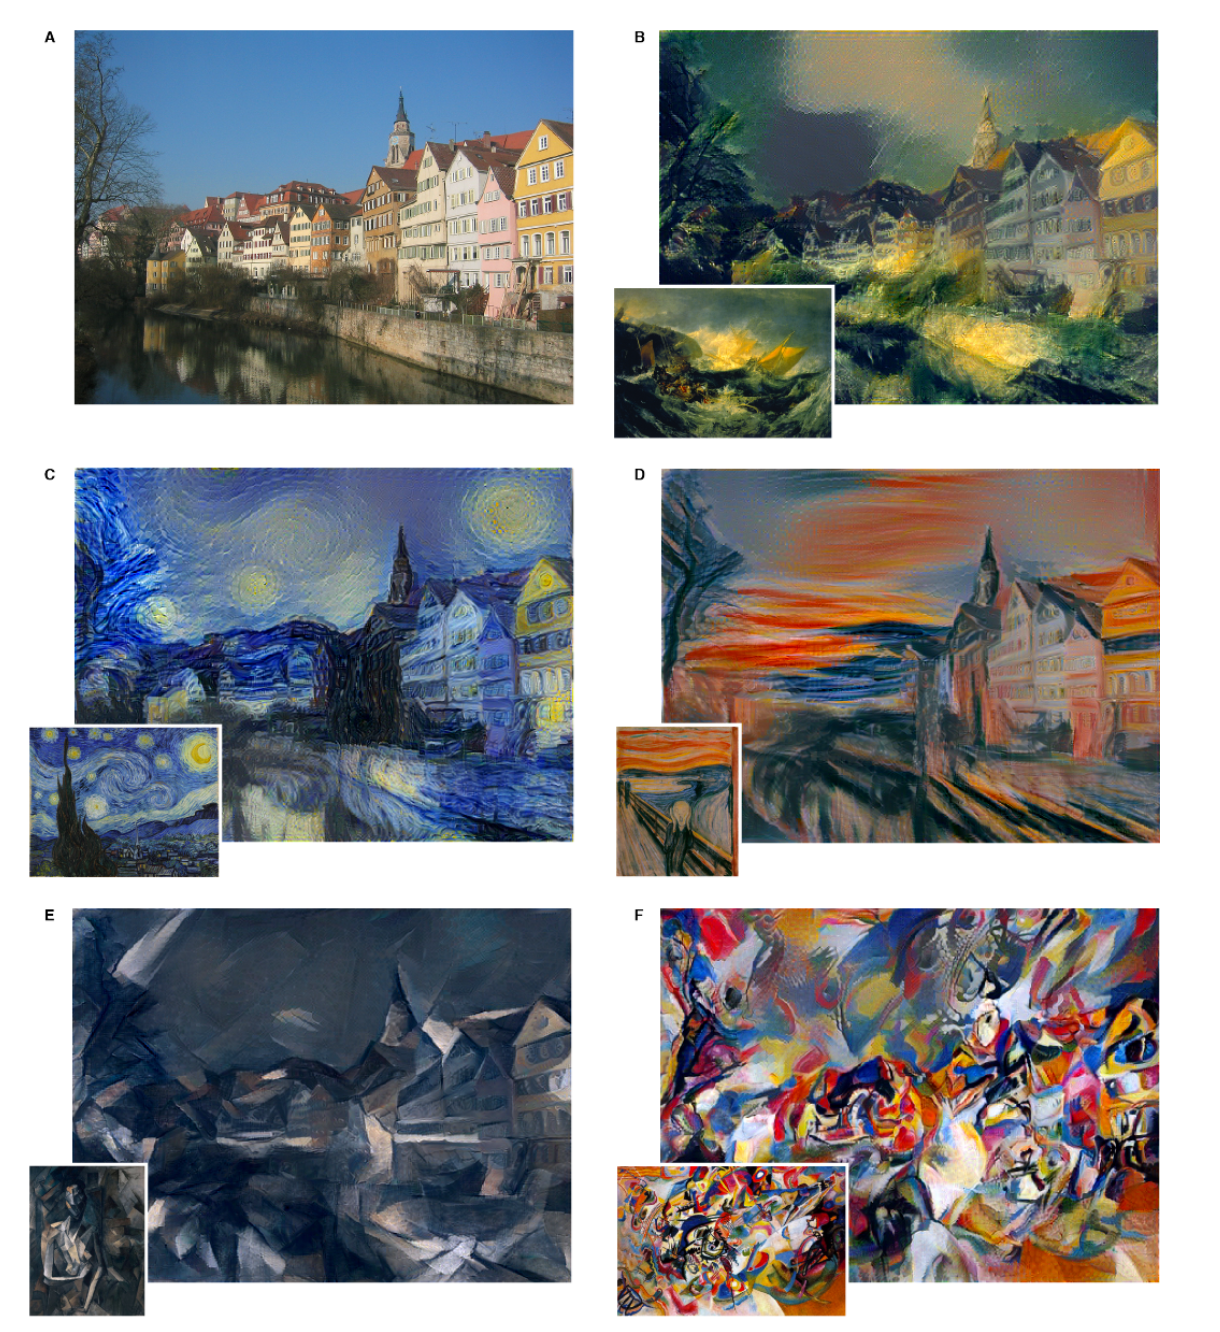
\includegraphics[width=0.5\textwidth]{nn_art_styles.png}
\caption{\label{fig:nn_art_styles} Application of various artistic styles to a content-image achieved through deep neural networks \cite{Gatys2015AStyle}} 
\end{figure}

While the fitness exhibited by biological systems (i.e. the high fitness of individual phenotypes) is indeed spectacular, another marvel of biology lurks just behind the parade of sundry phenotypes well-suited to their respective environments: the genotype-phenotype mapping. Although this mapping might be naively dismissed as a mere implementation detail, it contributes to a number of properties essential to the evolutionary process. Among others, these include modularity, neutrality, robustness, weak linkage, and degeneracy \cite{Richter2015EvolvabilitySurvey, DowningIntelligenceSystems}.  The genotype-phenotype mapping reorganizes the evolutionary search space, placing relatively distant phenotypes in close evolutionary proximity. Consider Figure \ref{fig:arabidopsis_mutants}, which compares Wild Type \textit{Arabidopsis thaliana} with five mutant strains. These individuals are clustered together in the genotypic space of \textit{Arabidopsis thaliana}. Although the genotypic distance between these phenotypes is small, a relatively broad range of phenotypes is represented. While none of these the mutations would seem to confer selective advantage, they are representative of the rich diversity of form that is accessible to evolutionary search, allowing rapid adaptation to environmental changes or novel adaptation to the existing environment. Figure \ref{fig:arabidopsis_mutants} illustrates, in particular, the modularity of the system under genotype-phenotype mapping; the mutant strains exhibit significant variability in overall composition of the individual while preserving the general character of existing components. Although not illustrated in Figure \ref{fig:arabidopsis_mutants}, the local genotypic neighborhood also maps to a great number of phenotypes indistinguishable from Wild Type individuals, specimens that differ by more calibration-like adjustments to various properties of form, as well as -- doubtlessly -- fundamentally defective phenotypes. Further, the phenotype (for the most part) is known to exhibit stability under ordinary operations on the genetic space, such as recombination via crossover.

Although the importance of the genotype-phenotype mapping is non-obvious when considering the phenotypes of individuals in isolation, its importance becomes clear when viewing them in the larger evolutionary context of life: the genotype-phenotype mapping made the phenotypic forms observed in nature accessible to the evolutionary process in the first place. If the evolutionary search space were not reorganized by the genotype-phenotype mapping, the evolutionary search would be stymied.  Take, for example, the repetition of structure at the very root of the cellular nature of life, the symmetries of biological forms, or the surprising  reapplications of existing mechanisms (such as ion flows in neural signaling), all of which would almost certainly be inaccessible in a phenotype-based search space.

This project will investigate how genotype-phenotype mapping induces evolvability -- ultimately, making high-fitness individuals accessible via evolutionary search -- in the context of artificial neural networks. That is, investigating how different methods of generating network structure from a genetic encoding (which is operated on by mutation and recombination) affects the viability of evolutionary search for an ANN to perform a certain task. It is hoped that, although perhaps not through this individual piece of work, this line of inquiry will ultimately contribute to the development of more capable and versatile artificial intelligence systems.

\begin{figure}
\centering
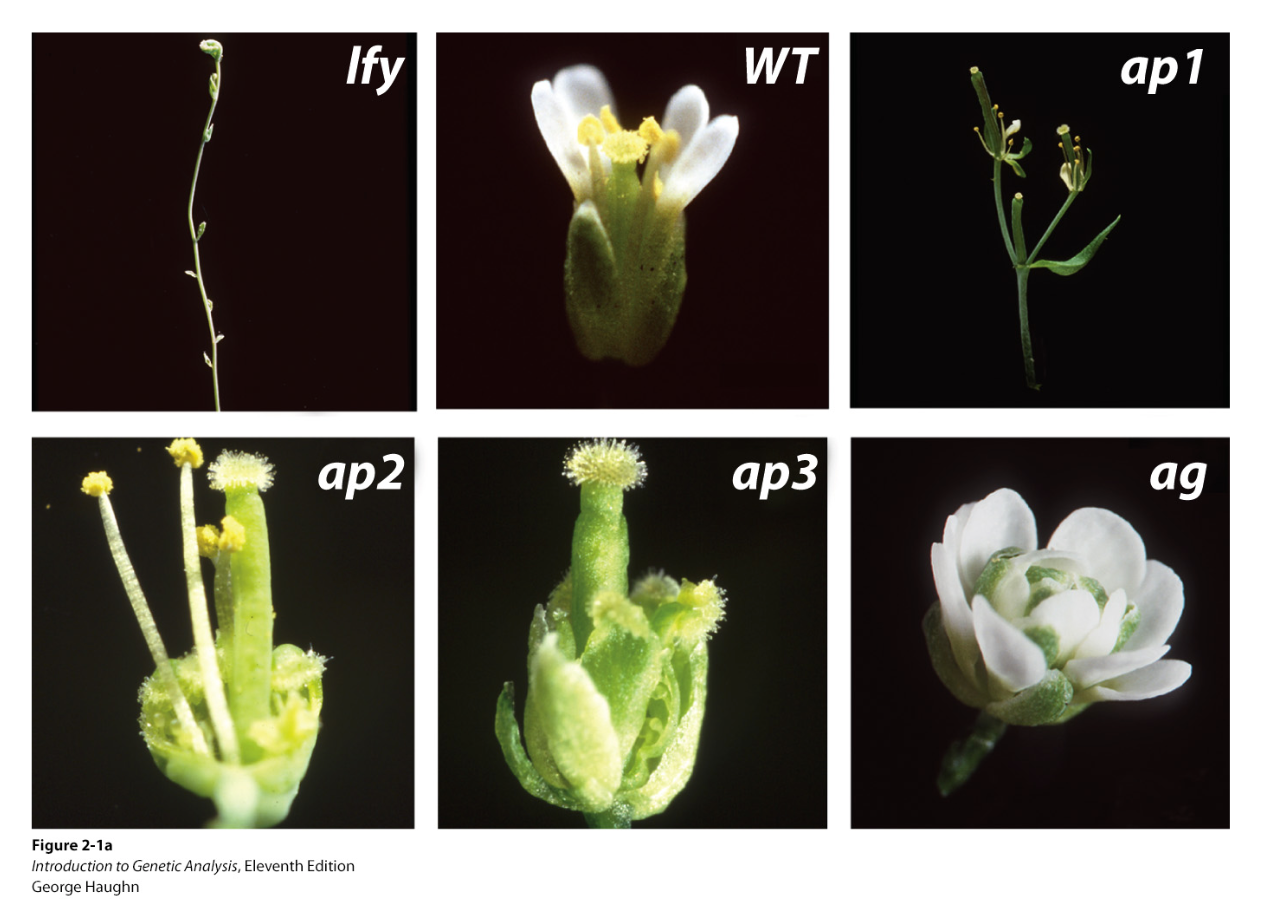
\includegraphics[width=0.6\textwidth]{arabidopsis_mutations.png}
\caption{\label{fig:arabidopsis_mutants}Wild-type and mutant strains of \textit{Arabidopsis thaliana} \cite{Griffiths2015IntroductionAnalysis}} 
\end{figure}